\section{moeo\-Additive\-Epsilon\-Binary\-Metric$<$ Objective\-Vector $>$ Class Template Reference}
\label{classmoeoAdditiveEpsilonBinaryMetric}\index{moeoAdditiveEpsilonBinaryMetric@{moeoAdditiveEpsilonBinaryMetric}}
Additive epsilon binary metric allowing to compare two objective vectors as proposed in Zitzler E., Thiele L., Laumanns M., Fonseca C.  


{\tt \#include $<$moeo\-Additive\-Epsilon\-Binary\-Metric.h$>$}

Inheritance diagram for moeo\-Additive\-Epsilon\-Binary\-Metric$<$ Objective\-Vector $>$::\begin{figure}[H]
\begin{center}
\leavevmode
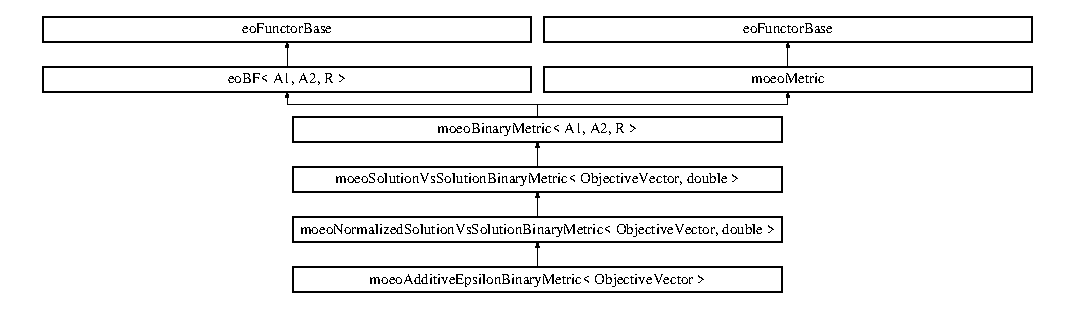
\includegraphics[height=3.70044cm]{classmoeoAdditiveEpsilonBinaryMetric}
\end{center}
\end{figure}
\subsection*{Public Member Functions}
\begin{CompactItemize}
\item 
double \bf{operator()} (const Objective\-Vector \&\_\-o1, const Objective\-Vector \&\_\-o2)
\begin{CompactList}\small\item\em Returns the minimal distance by which the objective vector \_\-o1 must be translated in all objectives so that it weakly dominates the objective vector \_\-o2. \item\end{CompactList}\end{CompactItemize}
\subsection*{Private Member Functions}
\begin{CompactItemize}
\item 
double \bf{epsilon} (const Objective\-Vector \&\_\-o1, const Objective\-Vector \&\_\-o2, const unsigned int \_\-obj)
\begin{CompactList}\small\item\em Returns the epsilon value by which the objective vector \_\-o1 must be translated in the objective \_\-obj so that it dominates the objective vector \_\-o2. \item\end{CompactList}\end{CompactItemize}


\subsection{Detailed Description}
\subsubsection*{template$<$class Objective\-Vector$>$ class moeo\-Additive\-Epsilon\-Binary\-Metric$<$ Objective\-Vector $>$}

Additive epsilon binary metric allowing to compare two objective vectors as proposed in Zitzler E., Thiele L., Laumanns M., Fonseca C. 

M., Grunert da Fonseca V.: Performance Assessment of Multiobjective Optimizers: An Analysis and Review. IEEE Transactions on Evolutionary Computation 7(2), pp.117\^{a}��132 (2003). 



Definition at line 49 of file moeo\-Additive\-Epsilon\-Binary\-Metric.h.

\subsection{Member Function Documentation}
\index{moeoAdditiveEpsilonBinaryMetric@{moeo\-Additive\-Epsilon\-Binary\-Metric}!operator()@{operator()}}
\index{operator()@{operator()}!moeoAdditiveEpsilonBinaryMetric@{moeo\-Additive\-Epsilon\-Binary\-Metric}}
\subsubsection{\setlength{\rightskip}{0pt plus 5cm}template$<$class Objective\-Vector$>$ double \bf{moeo\-Additive\-Epsilon\-Binary\-Metric}$<$ Objective\-Vector $>$::operator() (const Objective\-Vector \& {\em \_\-o1}, const Objective\-Vector \& {\em \_\-o2})\hspace{0.3cm}{\tt  [inline]}}\label{classmoeoAdditiveEpsilonBinaryMetric_545aa2c8e6dd93084276763c9d8a3709}


Returns the minimal distance by which the objective vector \_\-o1 must be translated in all objectives so that it weakly dominates the objective vector \_\-o2. 

\begin{Desc}
\item[Warning:]don't forget to set the bounds for every objective before the call of this function \end{Desc}
\begin{Desc}
\item[Parameters:]
\begin{description}
\item[{\em \_\-o1}]the first objective vector \item[{\em \_\-o2}]the second objective vector \end{description}
\end{Desc}


Definition at line 60 of file moeo\-Additive\-Epsilon\-Binary\-Metric.h.

References moeo\-Additive\-Epsilon\-Binary\-Metric$<$ Objective\-Vector $>$::epsilon().\index{moeoAdditiveEpsilonBinaryMetric@{moeo\-Additive\-Epsilon\-Binary\-Metric}!epsilon@{epsilon}}
\index{epsilon@{epsilon}!moeoAdditiveEpsilonBinaryMetric@{moeo\-Additive\-Epsilon\-Binary\-Metric}}
\subsubsection{\setlength{\rightskip}{0pt plus 5cm}template$<$class Objective\-Vector$>$ double \bf{moeo\-Additive\-Epsilon\-Binary\-Metric}$<$ Objective\-Vector $>$::epsilon (const Objective\-Vector \& {\em \_\-o1}, const Objective\-Vector \& {\em \_\-o2}, const unsigned int {\em \_\-obj})\hspace{0.3cm}{\tt  [inline, private]}}\label{classmoeoAdditiveEpsilonBinaryMetric_04253f76c832d24a3fd6bc574be54c46}


Returns the epsilon value by which the objective vector \_\-o1 must be translated in the objective \_\-obj so that it dominates the objective vector \_\-o2. 

\begin{Desc}
\item[Parameters:]
\begin{description}
\item[{\em \_\-o1}]the first objective vector \item[{\em \_\-o2}]the second objective vector \item[{\em \_\-obj}]the index of the objective \end{description}
\end{Desc}


Definition at line 89 of file moeo\-Additive\-Epsilon\-Binary\-Metric.h.

References moeo\-Normalized\-Solution\-Vs\-Solution\-Binary\-Metric$<$ Objective\-Vector, double $>$::bounds.

Referenced by moeo\-Additive\-Epsilon\-Binary\-Metric$<$ Objective\-Vector $>$::operator()().

The documentation for this class was generated from the following file:\begin{CompactItemize}
\item 
moeo\-Additive\-Epsilon\-Binary\-Metric.h\end{CompactItemize}
